\begin{figure}[t]
  \centering
   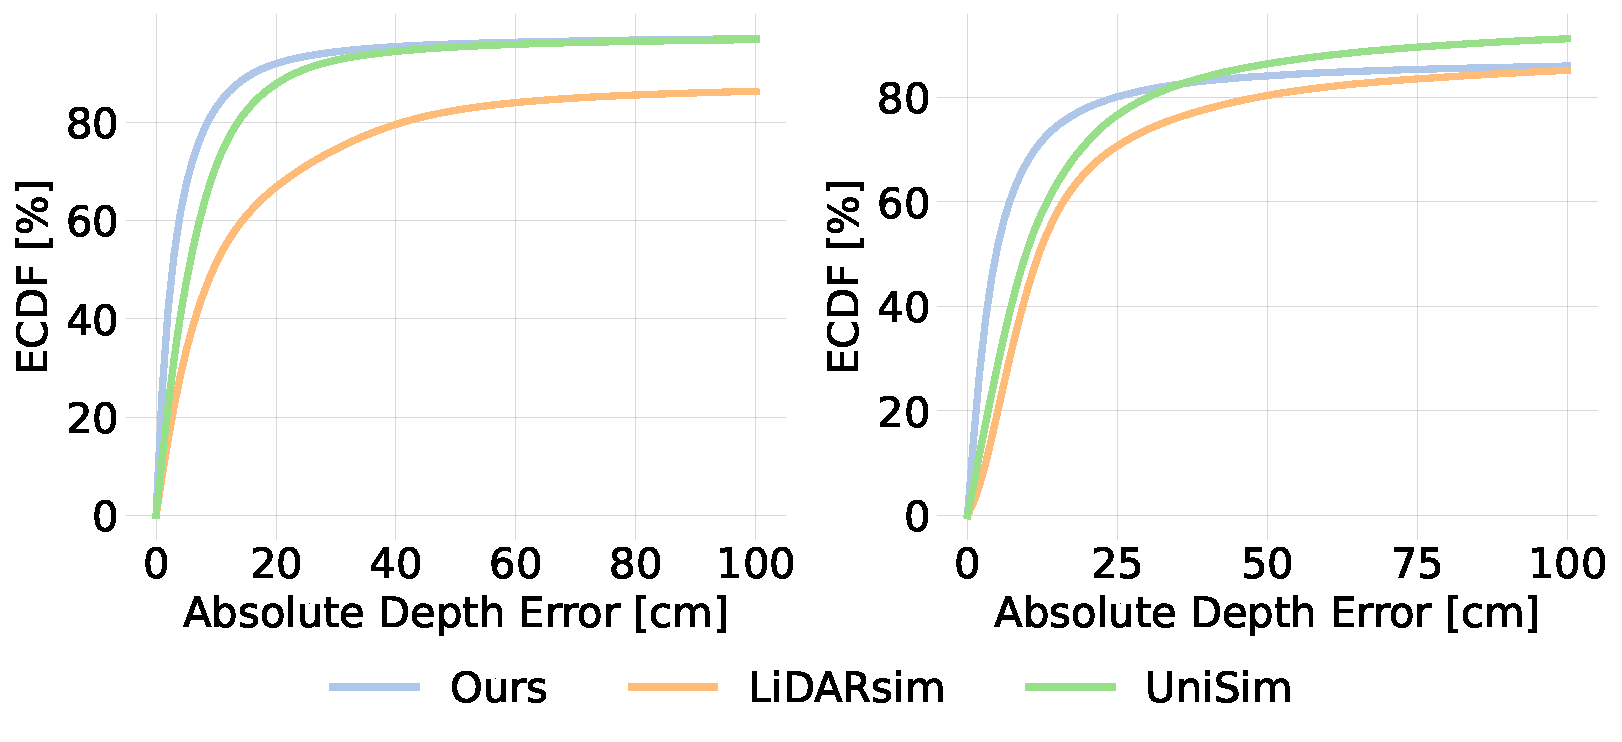
\includegraphics[width=1\columnwidth]{Figures/ecdf_3_methods.pdf}
   
        % \caption{On \textit{Waymo Dynamic}, ECDFs of our method, LiDARsim~\cite{manivasagam2020lidarsim}, and our method with our decomposition module replaced by the one in UniSim~\cite{yang2023unisim}. The left diagram represents the ECDF for all LiDAR measurements, while the right diagram represents the ECDF for measurements on dynamic vehicles only.}
        \caption{ECDF plots showcasing range errors across all the points (left) and specifically for points associated with dynamic vehicles (right). Our neural fields composition demonstrates superior performance over LiDARsim~\cite{manivasagam2020lidarsim} and UniSim~\cite{yang2023unisim}, especially in the context of dynamic vehicles.}
   \label{fig:ecdf}
   
\end{figure}